\documentclass[]{scrartcl}
\fontfamily{cmr}
%opening
\title{X-Ray Crystallography}
\author{Jeremy K. Thaller}

%\usepackage{color} %erlaubt Farben
%\usepackage{graphicx}
%\usepackage{amsmath}
%\usepackage{subfig} 

\usepackage{amsmath} %Formeln
\usepackage{mathtools} %Formeln
\usepackage{physics} %Formeln, insb. braket-Notation
\usepackage[utf8]{inputenc} %deutsche Zeichen
%\usepackage[ngerman]{babel} %deutsche Rechtschreibung
%\usepackage[english]{babel}
\usepackage{colortbl} %bunte Tabellen mit zwei Farbbeispielen
\definecolor{tab-gray}{gray}{0.85}
\definecolor{lightgreen}{cmyk}{0.07,0.001,0.1,0.001}
\usepackage{multirow} %bessere Tabellen
\usepackage{tabularx} %bessere Tabellen mit zwei oft genutzten Befehlen
\newcolumntype{x}[1]{!{\centering\arraybackslash\vrule width #1}}
\newcolumntype{C}[1]{>{\centering\arraybackslash}p{#1}}
\usepackage{enumitem} %bessere Nummerieung
\usepackage{color} %erlaubt Farben
\usepackage{float} %erlaubt float-Objekte
\usepackage{graphicx} %ermöglicht das Einbinden von Graphiken
\usepackage{subfig} %ermöglicht mehrere Graphiken in einer
\usepackage[dvipsnames]{xcolor}


\usepackage{hyperref} %Makes clickable T.o.c.
\hypersetup{
	colorlinks=true, %set true if you want colored links
	linktoc=all,     %set to all if you want both sections and subsections linked
	allcolors = black %get rid of weird auto link highlighting
}
\usepackage[printonlyused]{acronym} %ermöglicht Abkürzungsverzeichnis und trägt dort nur im Text verwendete Abkürzungen ein
\usepackage{pdfpages} %erlaubt Einbinden von pdfs als ganze Seiten
\usepackage{setspace} %besseres Format
\usepackage{geometry} %besseres Format mit Beispielseinstellungen
\geometry{a4paper, top=30mm, left=25mm, right=25mm, bottom=35mm,
	headsep=5mm, footskip=12mm}
\usepackage{array,booktabs,multirow}
\usepackage{upgreek}
\usepackage{chemmacros}
\usepackage{rotating}

%\renewcommand*{\familydefault}{\sfdefault}
\newcommand*{\head}{\bfseries}

%\usepackage[utf8]{inputenc}
%\usepackage[english]{babel}
%\usepackage{biblatex}
%\addbibresource{bibliography.bib} %Datei mit Quellen


\newcolumntype{_}{>{\global\let\currentrowstyle\relax}}
\newcolumntype{^}{>{\currentrowstyle}}
\newcommand{\rowstyle}[1]{\gdef\currentrowstyle{#1}%
	#1\ignorespaces
}
\begin{document}

\maketitle

\begin{abstract}

\end{abstract}


\section{Preliminary Information}
In this report, the structure of Ca\textsubscript{5}F\textsubscript{0.96}Cl\textsubscript{0.04}(PO\textsubscript{4})\textsubscript{3} (Apatite) with formula units per unit cell of $Z=2$ was investigated. In exercise 2, we determined that due to absorption effects, the maximum spherical size for a single crystal that may be used for x-ray diffraction using Cu-$ K_\alpha $ is $ 108\mu $m. The density of this crystal is 504.9 g/mol.


\section{XRD Background Theory}
The goal of x-ray diffraction crystallography (XRD) is to determine the structure of a given material by means of subjecting it to x-ray radiation. Any given atom in a crystal lattice will elastically scatter (diffract) the incoming photons according to Bragg's law (eq. \ref{bragg_law}), so long as the wavelength is not such that the electrons absorb and re-emit the incoming photon. This would be inelastic scattering and is the reason high energy x-rays are used in XRD.
\begin{equation}\label{bragg_law}
n\lambda = 2d_{hkl}\sin{\theta}
\end{equation}
The measured intensities of the scattered photons are proportional to the absolute value of the structure factor, $ F_{hkl} $, squared, as well as several correction terms, including the polarization factor, a geometric factor, and an absorption coefficient. The structure factor is the Fourier transform of the electronic density, and can be calculated as follows:
\begin{equation}
\label{struct_fact}
F_{hkl} = \sum_{j=1}^{N} f_j \exp[2\pi i(hx_j+ky_j+lz_j)]\textrm{.}
\end{equation}
Here, $ f_j $ is the scattering factor for atom j, which largely depends on the number of electrons contained by the atom. One can calculate the Intensities from the structure factor, but not vice versa, as the phase information is lost. Only the magnitude of $ F_{hkl} $ can be calculated from the intensities. Unfortunately, the detector only measures intensities. To find the atomic positions, we must first recover the structure factors using a pre-existing model, essentially a preliminary guess to check self-consistency. The structure factor then allows us to calculate the electronic densities, $ \rho(x,y,z) $ via equation (\ref{rho}), which in turn, leads to the atomic positions.

\begin{equation}\label{rho}
\rho(x,y,z) = \frac{1}{V} \sum_{h,k,l} F_{hkl} \exp \left[-2 \pi i \left( h\frac{x}{a}+k\frac{y}{b}+l\frac{z}{c}\right) \right]
\end{equation}

\subsection{Patterson Method}
Patterson synthesis is useful in structural determination, because it only requires knowing the magnitude of the structure factor, $ |F_{hkl}|, $ which we can calculate from the measured intensities and the aforementioned correction factors. The Patterson function is defined as: \begin{equation}\label{Patt}
P(u,v,w) = \sum_{h,k,l}|F_{hkl}|^2 e^{-2\pi i(hu+kv+lw)} \textrm{.}
\end{equation}

$ P(u,v,w) $ will have the largest peaks wherever $ p(x,y,z) $ is also the largest, thus the Patterson peaks correspond to electronic densities, and the highest peaks will correspond to the largest atoms (largest in the sense of greatest having more electrons and thus a higher atomic number). Thus, the distances between the Patterson peaks correspond to interatomic spacing; for materials with a few heavier atoms present, this method is especially useful. Comparing interatomic distances to those of the starting model allows for the determination of atomic positions. 

\subsection{Direct Determination Method}
To recover the lost phase information in the structure factor, we can calculate the normalized structure factor, $ E_{hkl} $, and determine if the structure is centrosymmetric via equation \ref{centro_cases}. 

\begin{equation}\label{scale}
E^2_{hkl} = \frac{F^2_{hkl}}{\langle F^2_{hkl} \rangle}
\end{equation}

\begin{equation}\label{centro_cases}
{\langle \ | E_{hkl}^2-1 | \ \rangle} = \begin{cases}0.968~\textrm{centrosymmetric}\\0.736 \textrm{~non-centrosymmetric}\end{cases}
\end{equation}
In 1952, American physicist David Sayre introduced an equation that allows for the calcualtion of structure factor phases for some reflections based on known structure factors. 

\begin{equation}
\label{sayre}
F_{hkl} = \sum_{h'k'l'} F_{h'k'l'} \cdot F_{h-h',k-k',l-l'}
\end{equation}
For centrosymmetric structures the phases can only be 0 or $ \pi $, so the Sayre equation can be reduced even further. The goal of structure refinement is the minimize difference between the calculated structure factor and the model, i.e. $ \Delta_1 = |F_0|-|F_c| $ and $ \Delta_2 = | F_{0}^2 - F_{c}^2 |$, using the least squares method.

\subsection{Least Squares Method}
To calculate the error for each iteration of model improvement, the least squares method is used. The loss function is calculated as the sum of the squared differences of model positions and the measured positions (residuals). The sum of the squared residuals for the x,y,and z positions are written in eq. \ref{least_sq}, where n are the total number of atoms considered. $ x_{calc}$ , $y_{calc}$ , and $z_{calc} $ are all functions of parameters that can be tweaked between iterations to minimize the loss.

\begin{equation}\label{least_sq}
s_x = \sum_{i=1}^n \left(x_{calc} - x_{model}\right)^2, \ s_y = \sum_{i=1}^n \left(y_{calc} - y_{model}\right)^2, \ s_z = \sum_{i=1}^n \left(z_{calc} - z_{model}\right)^2
\end{equation}

\subsection{Bond Valence Sums}
After fitting the atomic positions, we can calculate the bond valence sum (BVS) using the interatomic distances from the Patterson fitting. The BVS is the sum of all the bond valences ($ S_{ij} $), where each bond valence depends on its distance from other atoms and two constant parameters, $ R_0 $ and $ B $  (eq. \ref{bvs}).

\begin{equation}\label{bvs}
S_{ij} = exp\left[\frac{(R_0 - R_{ij})}{B} \right]
\end{equation}

\section{Sample Preparation and Data Collection}
First we cleaned a glass coverslip and placed a drop of DI water on it. Then we added a few crystals into the water, and scraped a few single crystals away in order to choose a one closest to the maximum allowed size for the diffraction. To mount the crystal for experimentation, we placed some putty in a heavy cylinder and inserted a thin needle through. Next, we added some glue on the tip of the needle and attached the chosen grain. We then placed the mounted sample into the x-ray diffractometer and adjusted the screws while rotating between the 0,90,180, and 270 degree positions to ensure the crystal was centered throughout its entire rotation on the view finder. 

Data was collected over a period of 21 hours with a $ \Delta\phi $ of $0.5^{\circ} $.

%\section{Data Reduction and Integration}
%The first step of data reduction is to find the location of the spots produced by the diffracted x-ray beam in the format of (x,y,$ \phi $). The is a two dimension curved structure with the h,k,l intensities distributed over the slice. First we unwarped the located spots and saved an image for each layer. 
%
%Next we manually reduced our data. \textit{....... Talk about the steps and things needed to change here? ........}
%
%Next, we use indexing to find the the h,k,l values. This will give us the unit cell and orientation. Next we refine this process, taking into account the detector distance, beam center, and mosaicity. 
%
%With this data processed, we now reach the integration stage. Here we predict reflection positions. We then assign pixels to the peak and the background, summing the peaks and subtracting the background. Every spot, i.e. an $ (h,k,l) $ coordinate) is summed to give an intensity, $ I_{hkl} $ for each. 


\section{Resulting Structure}
The calculated $(E_{\textrm{hkl}}^2-1)$ value was 0.974 and the determined space group was $ 176 (6_3/\text{m}) $. 

%\begin{figure}[h]
%	\centering
%	\includegraphics[width=0.7\linewidth]{files-to-include/hk0}
%	\caption[hko]{The hk0 plane as determine by the manual unwarping process.}
%	\label{fig:hk0}
%\end{figure}

\begin{figure}[h]
	\centering
	\subfloat[hk0 plane]{\includegraphics[scale=0.15]{{files-to-include/hk0}}}
	\qquad
	\subfloat[2kl plane]{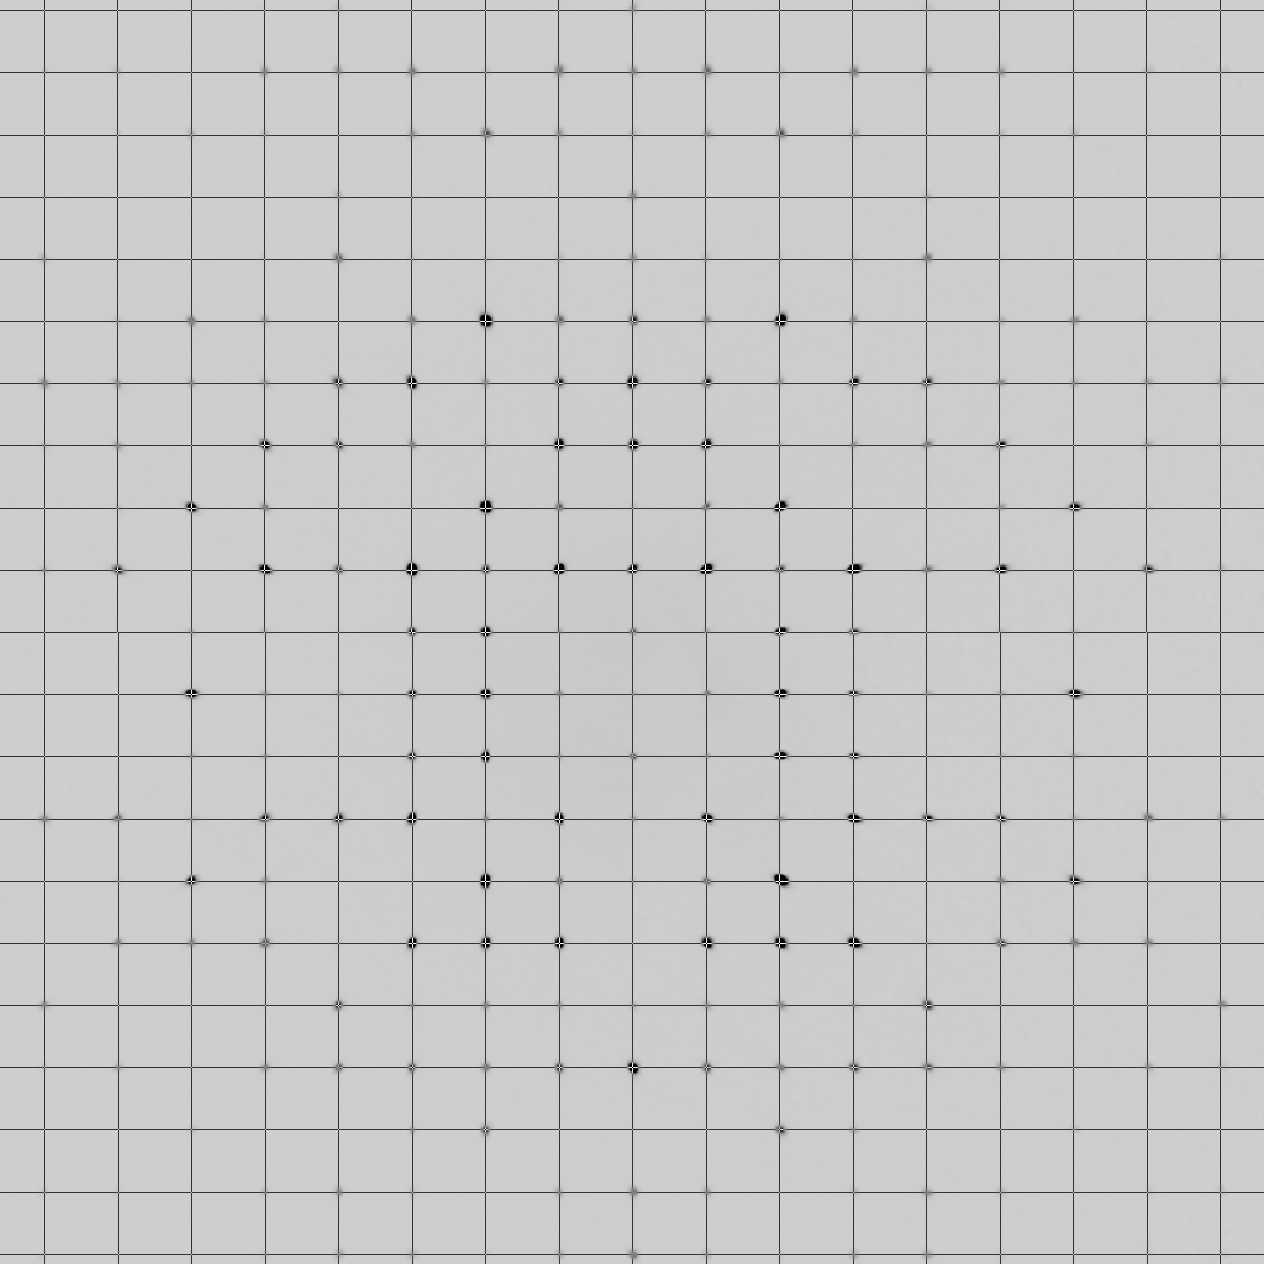
\includegraphics[scale=0.15]{{files-to-include/2kl}}}
	\caption[2kl plane]{Here are two different hkl planes}
	\label{hkl}
\end{figure}

\begin{figure}[h]
	\centering
	\subfloat[along c direction]{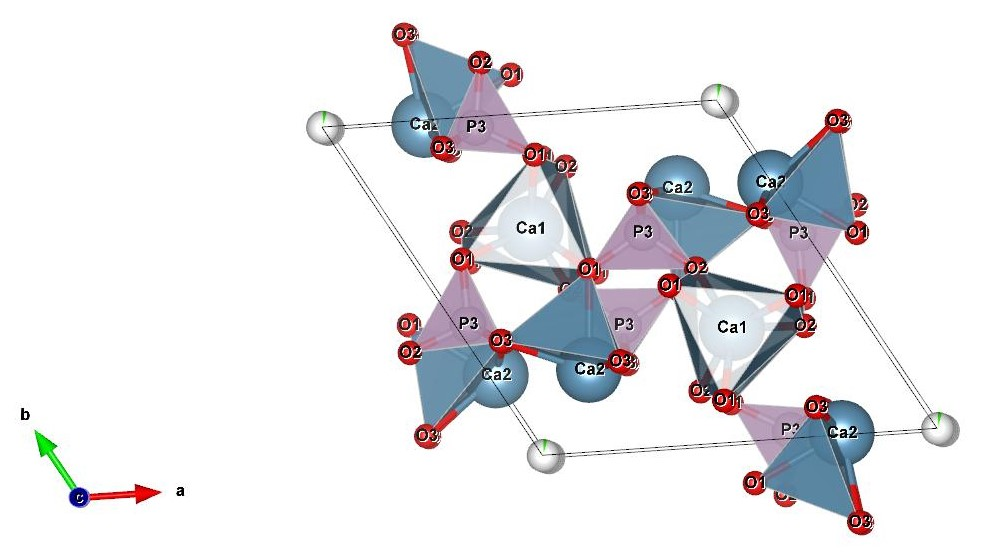
\includegraphics[scale=0.32]{{files-to-include/gr5ap_nice_cropped}}}
	\qquad
	\subfloat[along a direction]{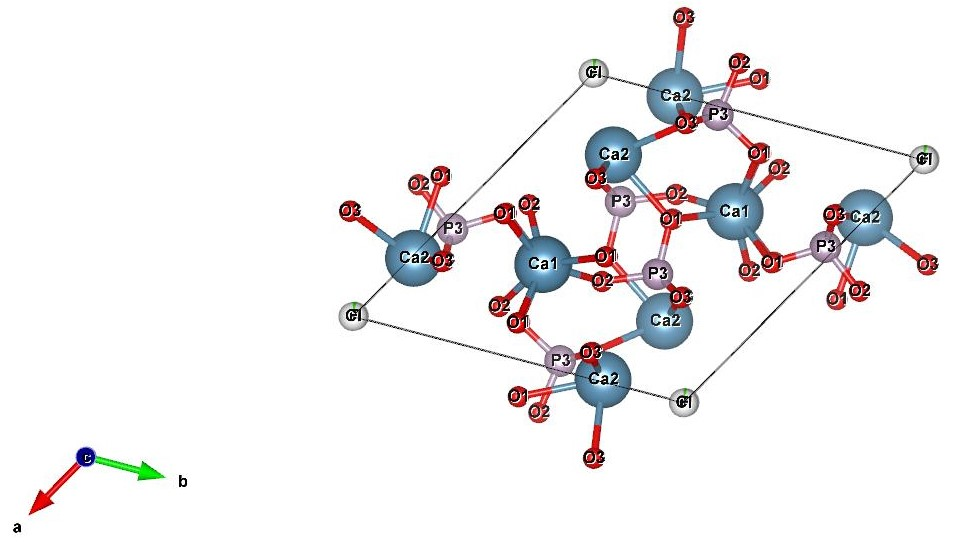
\includegraphics[scale=0.32]{{files-to-include/gr5apIIc_cropped}}}
	\caption[2kl plane]{Here are two views of the same structure generated by VESTA. In case the labels are too small to read, white is O, red is H, blue is Ca and purple is P.}
	\label{vesta}
\end{figure}

\begin{table}[H]
	\centering
	\caption[Cell parameters]{Below are the cell parameters calculated by \emph{CrysAlisPro}.}
	\begin{minipage}{0.45\textwidth}
		\centering
		\begin{tabular}{c|c}
			\cellcolor{Salmon} Cell parameters & \cellcolor{Salmon} Value\\
			\midrule
			a & 9.3968(6)\,\AA\\
			b & 9.3968(6)\,\AA\\
			c & 6.8854(0)\,\AA\\
			$\alpha$ & 90.000(0)° \\
			$\beta$ & 90.000(0)° \\
			$\gamma$ & 120.000(0)° \\
			Volume & 526.53266(6)\,\AA\textsuperscript{3}\\
		\end{tabular}\label{param}
	\end{minipage}
\end{table}

\begin{table}[H]
	\caption{Below are the calculated BVS values of the cations calculated via modification of the excel sheet made in the final exercise of this course.}
	\footnotesize
	\centering
	\begin{tabular}{|c|c|c|c|}
		\multicolumn{2}{c}{\cellcolor{Aquamarine} Direct method} & \multicolumn{2}{c}{\cellcolor{LimeGreen} Patterson method}\\
		\hline
		\textbf{Cation} &\textbf{ BVS} & \textbf{Cation}& \textbf{BVS}\\
		\hline
		Ca\_1 & 1.8650 & Ca\_1 & 1.8651\\
		\hline
		Ca\_2 & 2.0275 & Ca\_2 & 2.0334\\
		\hline
		P & 4.9791 & P & 4.9788\\
		\hline
	\end{tabular}\label{bvs}
\end{table}

\begin{table}[H]
	\centering
	\caption[Atomic positions]{Here are the atomic positions calculated by both the direct method and the Patterson method.}
	\begin{tabular}{c|c|c|c|c|c|c|c}
		&&\multicolumn{3}{c}{\cellcolor{Aquamarine} Direct method} & \multicolumn{3}{c}{\cellcolor{LimeGreen} Patterson method}\\
		\midrule
		Atom & Wyckoff position & x & y & z & x & y & z \\
		Ca\_1 & 6h & 0.249206 & 0.242123 & 0.250000 & 0.750796 & 0.757878 & 0.250000 \\
		\hline 
		\textit{error} & \ &  0.00812  &  0.00000  &  0.00000 &  0.00812  &  0.00000  &  0.00000   \\ 
		\hline
		
		Ca\_2 & 4f & 0.666667 & 0.333333 & 0.001163 & 0.333333 & 0.666667 & 0.498836 \\
		\hline
		\textit{error} & \ & 0.00731  &  0.00000 &   0.00000 & 0.00731  &  0.00000  &  0.00000 \\ 
		\hline
		P & 6h & 0.601526 & 0.0.630994 & 0.250000 & 0.970535 & 0.601526 & 0.250000 \\ 
		\hline
		\textit{error} & \ & 0.00696 &   0.00000 &   0.00000 & 0.00696 &   0.00000  &  0.00000 \\
		\hline
		F & 2a & 0.000000 & 0.000000 & 0.250000 & 1.000000 & 1.000000 & 0.250000 \\
		\hline
		\textit{error} & \ & 0.04734 &    0.00000 &   0.00000 & 0.04734 &   0.00000   & 0.00000 \\
		\hline 
		O\_1 & 6h & 0.412079 & 0.533297 & 0.250000 & 1.157439 & 0.672834 & 0.250000 \\
		\hline
		\textit{error} & \ & 0.02086 &   0.00000  &  0.00000 & 0.01258 &   0.00000 &   0.00000 \\
		\hline 
		O\_2 & 6h & 0.672833 & 0.515391 & 0.250000 & 0.878784 & 0.412081 & 0.250000 \\
		\hline
		\textit{error} & \ & 0.01258 &   0.00000 &   0.00000 & 0.02085 &   0.00000  &  0.00000 \\
		\hline 
		O\_3 & 12i & 0.658210 & 0.742762 & 0.070452 & 0.915447 & 0.658210 & 0.070446 \\
		\hline
		\textit{error} & \ & 0.01093 &    0.00460  &  0.00742 & 0.01092 &   0.00741  &  0.00282 \\
		\hline 
		Cl & 2a & 0.000000 & 0.000000 & 0.126183 & 1.000000 & 1.000000 & 0.125501 \\
		\hline
		\textit{error} & \ & 0.13024 &   0.00000 &   0.00000 & 1.000000  &   1.000000  &  0.125501 \\ 
		\hline
	\end{tabular}\label{atomicpos}
\end{table}




%\begin{table}[h!]
%	\centering
%	\small
%	\setlength\tabcolsep{1pt}
%	\resizebox{\columnwidth}{!}{
%	\begin{tabular}{|l|l|l|l|l|l|l|l|l|l|l|l|}
%		\hline
%		\multicolumn{1}{|c|}{\textbf{ATOM}} & \multicolumn{1}{c|}{\textbf{x}} & \multicolumn{1}{c|}{\textbf{y}} & \multicolumn{1}{c|}{\textbf{z}} & \multicolumn{1}{c|}{\textbf{sof}} & \multicolumn{1}{c|}{\textbf{U11}} & \multicolumn{1}{c|}{\textbf{U22}} & \multicolumn{1}{c|}{\textbf{U33}} & \multicolumn{1}{c|}{\textbf{U23}} & \multicolumn{1}{c|}{\textbf{U13}} & \multicolumn{1}{c|}{\textbf{U12}} & \multicolumn{1}{c|}{\textbf{Ueq}} \\ \hline
%		\textbf{Ca2}                        & 0.0122                          & 0.0085                          & 0.0081                          & 0.50000                           & 0.0108(8)                         & 0.01165(1)                        & 0.0081(3)                         & 0.00000                           & 0.00000                           & 0.007(10)                         & 0.0096(8)                         \\ \hline
%		\textbf{Ca1}                        & 0.0126                          & 0.0126                          & 0.0073                          & 0.33333                           & 0.01263(1)                        & 0.01263(1)                        & 0.0073(31)                        & 0.00000                           & 0.00000                           & 0.00632(5)                        & 0.0108(69)                        \\ \hline
%		\textbf{P3}                         & 0.0074                          & 0.0070                          & 0.0061                          & 0.50000                           & 0.0072(8)                         & 0.0067(815)                       & 0.0069(15)                        & 0.00000                           & 0.00000                           & 0.0039(12)                        & 0.00683(8)                        \\ \hline
%		\textbf{F}                          & 0.0482                          & 0.0099                          & 0.0099                          & 0.16000                           & 0.0099(34)                        & 0.0099(54)                        & 0.04818(56)                       & 0.00000                           & 0.00000                           & 0.00496(2)                        & 0.02268(4)                        \\ \hline
%		\textbf{O1}                         & 0.0209                          & 0.0120                          & 0.0081                          & 0.50000                           & 0.008(43)                         & 0.0111(8)                         & 0.02089(5)                        & 0.00000                           & 0.00000                           & 0.00425(3)                        & 0.01363(21)                       \\ \hline
%		\textbf{O2}                         & 0.0164                          & 0.0126                          & 0.0066                          & 0.50000                           & 0.01561(4)                        & 0.01183(4)                        & 0.01258(45)                       & 0.00000                           & 0.00000                           & 0.01019(41)                       & 0.01186(1)                        \\ \hline
%		\textbf{O3}                         & 0.0293                          & 0.0105                          & 0.0073                          & 1.00000                           & 0.026(31)                         & 0.0132(4)                         & 0.01094(35)                       & 0.0046(1)                         & 0.0074(31)                        & 0.0124(3)                         & 0.01570(7)                        \\ \hline
%		\textbf{Cl}                         & 0.1499                          & 0.0648                          & 0.0648                          & 0.01333                           & 0.06(481)                         & 0.06(480)                         & 0.149(90)                         & 0.00000                           & 0.00000                           & 0.032(40)                         & 0.093(17)                         \\ \hline
%	\end{tabular}}
%	\caption{Above are the calculated interatomic from the direct method. The x,y,z values are principle mean squared atomic displacements}
%\end{table}

\begin{table}[]
	\centering
	\setlength\tabcolsep{2pt}
	\begin{tabular}{|l|l|l|l|l|l|l|l|l|l|l|l|}
		\hline
		\multicolumn{1}{|c|}{\textbf{ATOM} \cellcolor{Aquamarine}} & \multicolumn{1}{c|}{\cellcolor{Aquamarine} \textbf{x}} & \multicolumn{1}{c|}{\cellcolor{Aquamarine} \textbf{y}} & \multicolumn{1}{c|}{\cellcolor{Aquamarine} \textbf{z}} & \multicolumn{1}{c|}{\cellcolor{Aquamarine} \textbf{sof}} & \multicolumn{1}{c|}{\cellcolor{Aquamarine} \textbf{U11}} & \multicolumn{1}{c|}{\cellcolor{Aquamarine} \textbf{U22}} & \multicolumn{1}{c|}{\cellcolor{Aquamarine} \textbf{U33}} & \multicolumn{1}{c|}{\cellcolor{Aquamarine} \textbf{U23}} & \multicolumn{1}{c|}{\cellcolor{Aquamarine} \textbf{U13}} & \multicolumn{1}{c|}{\cellcolor{Aquamarine} \textbf{U12}} & \multicolumn{1}{c|}{\cellcolor{Aquamarine} \textbf{Ueq}} \\ \hline
		\textbf{Ca\_2}                        & 0.0122                          & 0.0085                          & 0.0081                          & 0.50000                           & 0.01088                           & 0.01165                           & 0.00813                           & 0.00000                           & 0.00000                           & 0.00700                           & 0.00962                           \\ \hline
		\textit{Ca\_2 Errors}                           &                                 &                                 &                                 & 0.00000                           & 0.00013                           & 0.00013                           & 0.00012                           & 0.00000                           & 0.00000                           & 0.00010                           & 0.00008                           \\ \hline
		\textbf{Ca\_1}                        & 0.0126                          & 0.0126                          & 0.0073                          & 0.33333                           & 0.01263                           & 0.01263                           & 0.00733                           & 0.00000                           & 0.00000                           & 0.00632                           & 0.01086                           \\ \hline
		\textit{Ca\_1 Errors}                           &                                 &                                 &                                 & 0.00000                           & 0.00011                           & 0.00011                           & 0.00015                           & 0.00000                           & 0.00000                           & 0.00005                           & 0.00009                           \\ \hline
		\textbf{P\_3}                         & 0.0074                          & 0.0070                          & 0.0061                          & 0.50000                           & 0.00728                           & 0.00678                           & 0.00698                           & 0.00000                           & 0.00000                           & 0.00394                           & 0.00683                           \\ \hline
		\textit{P\_3 Errors}                           &                                 &                                 &                                 & 0.00000                           & 0.00015                           & 0.00015                           & 0.00015                           & 0.00000                           & 0.00000                           & 0.00012                           & 0.00008                           \\ \hline
		\textbf{F}                          & 0.0482                          & 0.0099                          & 0.0099                          & 0.16000                           & 0.00993                           & 0.00993                           & 0.04818                           & 0.00000                           & 0.00000                           & 0.00496                           & 0.02268                           \\ \hline
		\textit{F Errors}                           &                                 &                                 &                                 & 0.00000                           & 0.00054                           & 0.00054                           & 0.00156                           & 0.00000                           & 0.00000                           & 0.00027                           & 0.00049                           \\ \hline
		\textbf{O\_1}                         & 0.0209                          & 0.0120                          & 0.0081                          & 0.50000                           & 0.00808                           & 0.01118                           & 0.02089                           & 0.00000                           & 0.00000                           & 0.00425                           & 0.01363                           \\ \hline
		\textit{0\_1 Errors}
		&                                 &                                 &                                 & 0.00000                           & 0.00043                           & 0.00045                           & 0.00055                           & 0.00000                           & 0.00000                           & 0.00037                           & 0.00021                           \\ \hline
		\textbf{O\_2}                         & 0.0164                          & 0.0126                          & 0.0066                          & 0.50000                           & 0.01561                           & 0.01183                           & 0.01258                           & 0.00000                           & 0.00000                           & 0.01019                           & 0.01186                           \\ \hline
		\textit{0\_2 Errors}                           &                                 &                                 &                                 & 0.00000                           & 0.00048                           & 0.00045                           & 0.00047                           & 0.00000                           & 0.00000                           & 0.00041                           & 0.00019                           \\ \hline
		\textbf{O\_3}                         & 0.0293                          & 0.0105                          & 0.0073                          & 1.00000                           & 0.02631                           & 0.01324                           & 0.01094                           & 0.00461                           & 0.00743                           & 0.01243                           & 0.01570                           \\ \hline
		\textit{0\_3 Errors}                           &                                 &                                 &                                 & 0.00000                           & 0.00042                           & 0.00034                           & 0.00035                           & 0.00028                           & 0.00031                           & 0.00032                           & 0.00017                           \\ \hline
		\textbf{Cl}                         & 0.1499                          & 0.0648                          & 0.0648                          & 0.01333                           & 0.06480                           & 0.06480                           & 0.14990                           & 0.00000                           & 0.00000                           & 0.03240                           & 0.09317                           \\ \hline
		\textit{Cl Errors}
		&                                 &                                 &                                 & 0.00000                           & 0.01132                           & 0.01132                           & 0.04008                           & 0.00000                           & 0.00000                           & 0.00566                           & 0.01386                           \\ \hline
	\end{tabular}
	\caption{Above are the calculated interatomic from the direct method. The x,y,z values are principle mean squared atomic displacements}
\end{table}


%\begin{table}[h!]
%		\centering
%		\small
%		\setlength\tabcolsep{1pt}
%		\resizebox{\columnwidth}{!}{
%		\begin{tabular}{|l|l|l|l|l|l|l|l|l|l|l|l|}
%		\hline
%		\multicolumn{1}{|c|}{\textbf{ATOM}} & \multicolumn{1}{c|}{\textbf{x}} & \multicolumn{1}{c|}{\textbf{y}} & \multicolumn{1}{c|}{\textbf{z}} & \multicolumn{1}{c|}{\textbf{sof}} & \multicolumn{1}{c|}{\textbf{U11}} & \multicolumn{1}{c|}{\textbf{U22}} & \multicolumn{1}{c|}{\textbf{U33}} & \multicolumn{1}{c|}{\textbf{U23}} & \multicolumn{1}{c|}{\textbf{U13}} & \multicolumn{1}{c|}{\textbf{U12}} & \multicolumn{1}{c|}{\textbf{Ueq}} \\ \hline
%		\textbf{Ca1}                        & 0.0126                          & 0.0126                          & 0.0073                          & 0.33333                           & 0.01263(1)                        & 0.01263(1)                        & 0.00732(5)                        & 0.00000                           & 0.00000                           & 0.00631(5)                        & 0.01086(9)                        \\ \hline
%		\textbf{Ca2}                        & 0.0122                          & 0.0085                          & 0.0081                          & 0.50000                           & 0.0108(8)                         & 0.01165(3)                        & 0.00813(2)                        & 0.00000                           & 0.00000                           & 0.007(10)                         & 0.00961(8)                        \\ \hline
%		\textbf{P3}                         & 0.0074                          & 0.0070                          & 0.0061                          & 0.50000                           & 0.0061(9)                         & 0.00728(5)                        & 0.00698(1)                        & 0.00000                           & 0.00000                           & 0.00334(2)                        & 0.00682(8)                        \\ \hline
%		\textbf{F}                          & 0.0482                          & 0.0099                          & 0.0099                          & 0.16000                           & 0.00992(4)                        & 0.0099(2)                         & 0.04819(15)                       & 0.00000                           & 0.00000                           & 0.00496(2)                        & 0.02268(4)                        \\ \hline
%		\textbf{O1}                         & 0.0209                          & 0.0119                          & 0.0081                          & 0.50000                           & 0.01076(4)                        & 0.00808(4)                        & 0.02088(5)                        & 0.00000                           & 0.00000                           & 0.00382(3)                        & 0.01363(21)                       \\ \hline
%		\textbf{O2}                         & 0.0164                          & 0.0126                          & 0.0066                          & 0.50000                           & 0.00707(41)                       & 0.01561(4)                        & 0.01258(7)                        & 0.00000                           & 0.00000                           & 0.00543(3)                        & 0.01186(19)                       \\ \hline
%		\textbf{O3}                         & 0.0293                          & 0.0105                          & 0.0073                          & 1.00000                           & 0.01469(3)                        & 0.02631(2)                        & 0.01094(35)                       & 0.00743(1)                        & 0.00282(2)                        & 0.01388(3)                        & 0.01570(7)                        \\ \hline
%		\textbf{Cl}                         & 0.1508                          & 0.0648                          & 0.0648                          & 0.01333                           & 0.06478(32)                       & 0.06(478)                         & 0.15(083)                         & 0.00000                           & 0.00000                           & 0.032(39)                         & 0.09(347)                         \\ \hline
%	\end{tabular}}
%		\caption{Above are the calculated interatomic from the Patterson method. The x,y,z values are principle mean squared atomic displacements. They identical in nearly all cases.}
%\end{table}

	\begin{table}[]
	\centering
	
	\setlength\tabcolsep{2pt}
	\begin{tabular}{|l|l|l|l|l|l|l|l|l|l|l|l|}
		\hline
		\multicolumn{1}{|c|}{\textbf{ATOM} \cellcolor{LimeGreen}} & \multicolumn{1}{c|}{\cellcolor{LimeGreen} \textbf{x}} & \multicolumn{1}{c|}{\cellcolor{LimeGreen} \textbf{y}} & \multicolumn{1}{c|}{\cellcolor{LimeGreen} \textbf{z}} & \multicolumn{1}{c|}{\cellcolor{LimeGreen} \textbf{sof}} & \multicolumn{1}{c|}{\cellcolor{LimeGreen} \textbf{U11}} & \multicolumn{1}{c|}{\cellcolor{LimeGreen} \textbf{U22}} & \multicolumn{1}{c|}{\cellcolor{LimeGreen} \textbf{U33}} & \multicolumn{1}{c|}{\cellcolor{LimeGreen} \textbf{U23}} & \multicolumn{1}{c|}{\cellcolor{LimeGreen} \textbf{U13}} & \multicolumn{1}{c|}{\cellcolor{LimeGreen} \textbf{U12}} & \multicolumn{1}{c|}{\cellcolor{LimeGreen} \textbf{Ueq}} \\ \hline
		\textbf{Ca\_1}                        & 0.0126                          & 0.0126                          & 0.0073                          & 0.33333                           & 0.01263                           & 0.01263                           & 0.00732                           & 0.00000                           & 0.00000                           & 0.00631                           & 0.01086                           \\ \hline
		\textit{Ca\_1 Errors}                           &                                 &                                 &                                 & 0.00000                           & 0.00011                           & 0.00011                           & 0.00015                           & 0.00731                           & 0.00000                           & 0.00005                           & 0.00009                           \\ \hline
		\textbf{Ca\_2}                        & 0.0122                          & 0.0085                          & 0.0081                          & 0.50000                           & 0.01088                           & 0.01165                           & 0.00813                           & 0.00000                           & 0.00000                           & 0.00700                           & 0.00961                           \\ \hline
		\textit{Ca\_2 Errors}                           &                                 &                                 &                                 & 0.00000                           & 0.00013                           & 0.00013                           & 0.00012                           & 0.00000                           & 0.00000                           & 0.00010                           & 0.00008                           \\ \hline
		\textbf{P\_3}                         & 0.0074                          & 0.0070                          & 0.0061                          & 0.50000                           & 0.00619                           & 0.00728                           & 0.00698                           & 0.00000                           & 0.00000                           & 0.00334                           & 0.00682                           \\ \hline
		\textit{P\_3 Errors}                           &                                 &                                 &                                 & 0.00000                           & 0.00015                           & 0.00015                           & 0.00015                           & 0.00000                           & 0.00000                           & 0.00012                           & 0.00008                           \\ \hline
		\textbf{F}                          & 0.0482                          & 0.0099                          & 0.0099                          & 0.16000                           & 0.00992                           & 0.00992                           & 0.04819                           & 0.00000                           & 0.00000                           & 0.00496                           & 0.02268                           \\ \hline
		\textit{F Errors}                           &                                 &                                 &                                 & 0.00000                           & 0.00054                           & 0.00054                           & 0.00156                           & 0.00000                           & 0.00000                           & 0.00027                           & 0.00049                           \\ \hline
		\textbf{O1}                         & 0.0209                          & 0.0119                          & 0.0081                          & 0.50000                           & 0.01076                           & 0.00808                           & 0.02088                           & 0.00000                           & 0.00000                           & 0.00382                           & 0.01363                           \\ \hline
		\textit{O\_1 Errors}
		&                                 &                                 &                                 & 0.00000                           & 0.00046                           & 0.00043                           & 0.00055                           & 0.00000                           & 0.00000                           & 0.00037                           & 0.00021                           \\ \hline
		\textbf{O2}                         & 0.0164                          & 0.0126                          & 0.0066                          & 0.50000                           & 0.00707                           & 0.01561                           & 0.01258                           & 0.00000                           & 0.00000                           & 0.00543                           & 0.01186                           \\ \hline
		\textit{O\_2 Errors}                           &                                 &                                 &                                 & 0.00000                           & 0.00041                           & 0.00048                           & 0.00047                           & 0.00000                           & 0.00000                           & 0.00038                           & 0.00019                           \\ \hline
		\textbf{O\_3}                         & 0.0293                          & 0.0105                          & 0.0073                          & 1.00000                           & 0.01469                           & 0.02631                           & 0.01094                           & 0.00743                           & 0.00282                           & 0.01388                           & 0.01570                           \\ \hline
		\textit{O\_3 Errors}                           &                                 &                                 &                                 & 0.00000                           & 0.00034                           & 0.00042                           & 0.00035                           & 0.00031                           & 0.00028                           & 0.00032                           & 0.00017                           \\ \hline
		\textbf{Cl}                         & 0.1508                          & 0.0648                          & 0.0648                          & 0.01333                           & 0.06478                           & 0.06478                           & 0.15083                           & 0.00000                           & 0.00000                           & 0.03239                           & 0.09347                           \\ \hline
		\textit{Cl Errors}
		&                                 &                                 &                                 & 0.00000                           & 0.01132                           & 0.01132                           & 0.04040                           & 0.00000                           & 0.00000                           & 0.00566                           & 0.01395                           \\ \hline
	\end{tabular}
	\caption{Above are the calculated interatomic from the Patterson method. The x,y,z values are principle mean squared atomic displacements. They identical in nearly all cases.}
\end{table}

\section{Discussion}
Figure \ref{hkl} shows excellent agreement with the determined space group, since both the bond angles angles and predicted systematic extinction are seen. These extinctions are a result of the $ 6_3 $ screw axis. Additionally, the spots in figure \ref{hkl} are well resolved and clear. The calculated ${\langle |E_{\textrm{hkl}}^2-1| \rangle}$ value of 0.974 is close to the predicted value of 0.968 for centrosymmetric structures (see equation \ref{centro_cases}). The direct method and Patterson methods both produce very similar results, another positive sign for an accurately determined structure. Because there is not a single particularly large atom present in the material, the direct determination method may be better.Both the direct and Patterson methods had a small R1 value of just 0.0202 (smaller indicates higher data quality). 


\bibliographystyle{IEEEtran}
\bibliography{bibliography}
\nocite{pat}
\nocite{expo2014}
\nocite{mit}
\nocite{ripoll}
\nocite{scidir}


%\bibliography{bibliography.bib} 

%%https://www.xtal.iqfr.csic.es/Cristalografia/parte_07_3-en.html
% Ripoll, Martin Martinez. The Patterson Function and the Patterson Method, www.xtal.iqfr.csic.es/Cristalografia/parte\_07\_3-en.html.
%\\
%%\hangindent=1em
%%\hangafter=1
%%http://www.bio.brandeis.edu/classes/archives/biochem102/sftut/frame_patt1.html
%The Patterson Function, www.bio.brandeis.edu/classes/archives/biochem102/sftut/frame\_patt1.html.
%\\
%%https://ocw.mit.edu/courses/chemistry/5-069-crystal-structure-analysis-spring-2010/lecture-notes/phasing_handout1.pdf
%“Phasing\_handout1.” Ocw.mit.edu, 2010, Spring, ocw.mit.edu/courses/chemistry/5-069-crystal-structure-analysis-spring-2010/lecture-notes/phasing\_handout1.pdf.
%\\
%%https://www.sciencedirect.com/topics/materials-science/x-ray-diffraction
%“X-Ray Diffraction.” X-Ray Diffraction - an Overview | ScienceDirect Topics, www.sciencedirect.com/topics/materials-science/x-ray-diffraction.
%\\
%“Bond Valence Sum.” Expo2014, www.ba.ic.cnr.it/softwareic/expo/bond-valence-sum/.

\end{document}
